\documentclass{article}

% Packages from Nicholas
\usepackage[english]{babel}
\usepackage[utf8]{inputenc}
\usepackage{fancyhdr}
\usepackage{amsmath}
\usepackage{amssymb}
\usepackage{bm}
\usepackage{geometry}
% \geometry{letterpaper}
\usepackage{amsfonts}
\usepackage{mathtools}
\usepackage{setspace}
\usepackage{makecell}
\usepackage{eurosym}
\usepackage{amstext}
\usepackage{framed}

% Inline Graphics
\usepackage{graphicx,float,subfig, grffile}
\graphicspath{{./}{figs/}}

% Captions
\usepackage[font=Large]{caption}

% Hypertext References
\usepackage{hyperref,color,textcomp}
\definecolor{webgreen}{rgb}{0,.35,0}
\definecolor{webbrown}{rgb}{.6,0,0}
\definecolor{RoyalBlue}{rgb}{0,0,0.9}
\definecolor{purp}{rgb}{0.6,0.3,0.9}
\hypersetup{
   colorlinks=true, linktocpage=true, pdfstartpage=3, pdfstartview=FitV,
   breaklinks=true, pdfpagemode=UseNone, pageanchor=true, pdfpagemode=UseOutlines,
   plainpages=false, bookmarksnumbered, bookmarksopen=true, bookmarksopenlevel=1,
   hypertexnames=true, pdfhighlight=/O,
   urlcolor=webbrown, linkcolor=RoyalBlue, citecolor=webgreen,
   pdfauthor={Nicholas Beasley, William Burke & Michael S. Emanuel},
   pdfsubject={Harvard AM205 (Fall 2018)},
   pdfkeywords={},
   pdfcreator={pdfLaTeX},
   pdfproducer={LaTeX with hyperref}
}
\hypersetup{pdftitle={AM205: Final Project}}

% Macro definitions
\newcommand{\N}{\mathbb{N}}
\newcommand{\Z}{\mathbb{Z}}
\newcommand{\Q}{\mathbb{Q}}
\newcommand{\R}{\mathbb{R}}
\newcommand{\B}{\mathbb{B}}
\newcommand{\mcL}{\mathcal{L}}
\newcommand{\p}{\partial}
\newcommand{\Trans}{\mathsf{T}}
\renewcommand{\vec}[1]{\mathbf{#1}}
\newcommand{\vx}{\vec{x}}
\newcommand{\vb}{\vec{b}}

\pagestyle{fancy}
\fancyhf{}
\chead{Basketball Motion Capture}
% \rhead{}
\rfoot{Page \thepage}
\lfoot{December 20, 2018}
\cfoot{}
\renewcommand{\headrulewidth}{0.5pt}
\renewcommand{\footrulewidth}{0.5pt}

\onehalfspacing
\begin{document}

\section*{AM205: Final Project}
\section*{Basketball Motion Capture}
\subsubsection*{Nicholas Beasley}
\subsubsection*{William C. Burke}
\subsubsection*{Michael S. Emanuel}

\section{Abstract}
The goal of this project was to infer the position of a basketball in three dimensional space during a live game by obtaining multiple video recordings.
In particular, the intuition was that with enough cameras, it should be possible to construct an over-determined system and perform 
a least squares or similar style estimation of the position of the ball that is in best agreement with the video frames.
Steps we hoped to achieve in this project included 
\begin{itemize}
\item obtaining video in an experiment at the MAC; processing the video; 
\item synchronizing the video based on the audio from each clip; 
\item mapping from 3D world coordinates to 2D pixel locations on each camera;
\item tracking the ball in 2D space on each camera; 
\item inferring the position of the ball in 3D space based on its pixel location on each camera.
\item simulating the path of the ball while in flight using an extended Kalman filter and the equations of motion
\item predicting whether a shot would go in the basket at the moment it was released
\end{itemize}

When we articulated this project, we recognized that it was ambitious and that it might not be possible to do everything we wanted to
in the time available.  It has turned out that a number of the steps, while conceptually straightforward, have proven to be quite
challenging and consumed far more time than we had budgeted.  We are going to present below everything that we were able
to accomplish and hope for the forbearance of readers who are familiar with the slings and arrows of working on demanding problems.

\section{Motivation}
Autonomous robots including autonomous vehicles are a field of major research activity and commercial interest.
One of the major open challenges in designing these robots is sensing their environments.
Autonomous driving systems on the road today have expensive and complex sensing systems
that often include multiple cameras and LIDAR.
This was one motivation behind the idea of attempting to solve a problem of perceiving the motion
of objects in a complicated environment that also included people.

Separate from any directly practical applications, basketball is one of the popular sports in both the US and the world.
The NBA had \$14 billion in revenues in 2017.  According to Wikipedia  it is the second most popular sport in the US
and has the highest participation.   
\footnote{\href{https://en.wikipedia.org/wiki/Sports_in_the_United_States}{sports in the united states}}
A practical system that would enable accurate 3D coordinate positions of the ball during live games might
attract considerable interest, both for entertainment and sports analytics.

\section{Experimental Set-Up}


\section{Conventions}
Coordinates in the world frame will be denoted as $(U, V, W)$. Coordinates in the camera frame will be denoted as $(X, Y, Z)$. Coordinates in the 2D image plane will be denoted as $(x, y)$. Pixel coordinates will be denoted as $(u, v)$. \\

The court has the following dimensions and coordinate system (all units are in FEET for this project). Note that we are centering the world coordinate system at the center of the court and that the $w$ axis points towards the ceiling.

\begin{figure}[H]
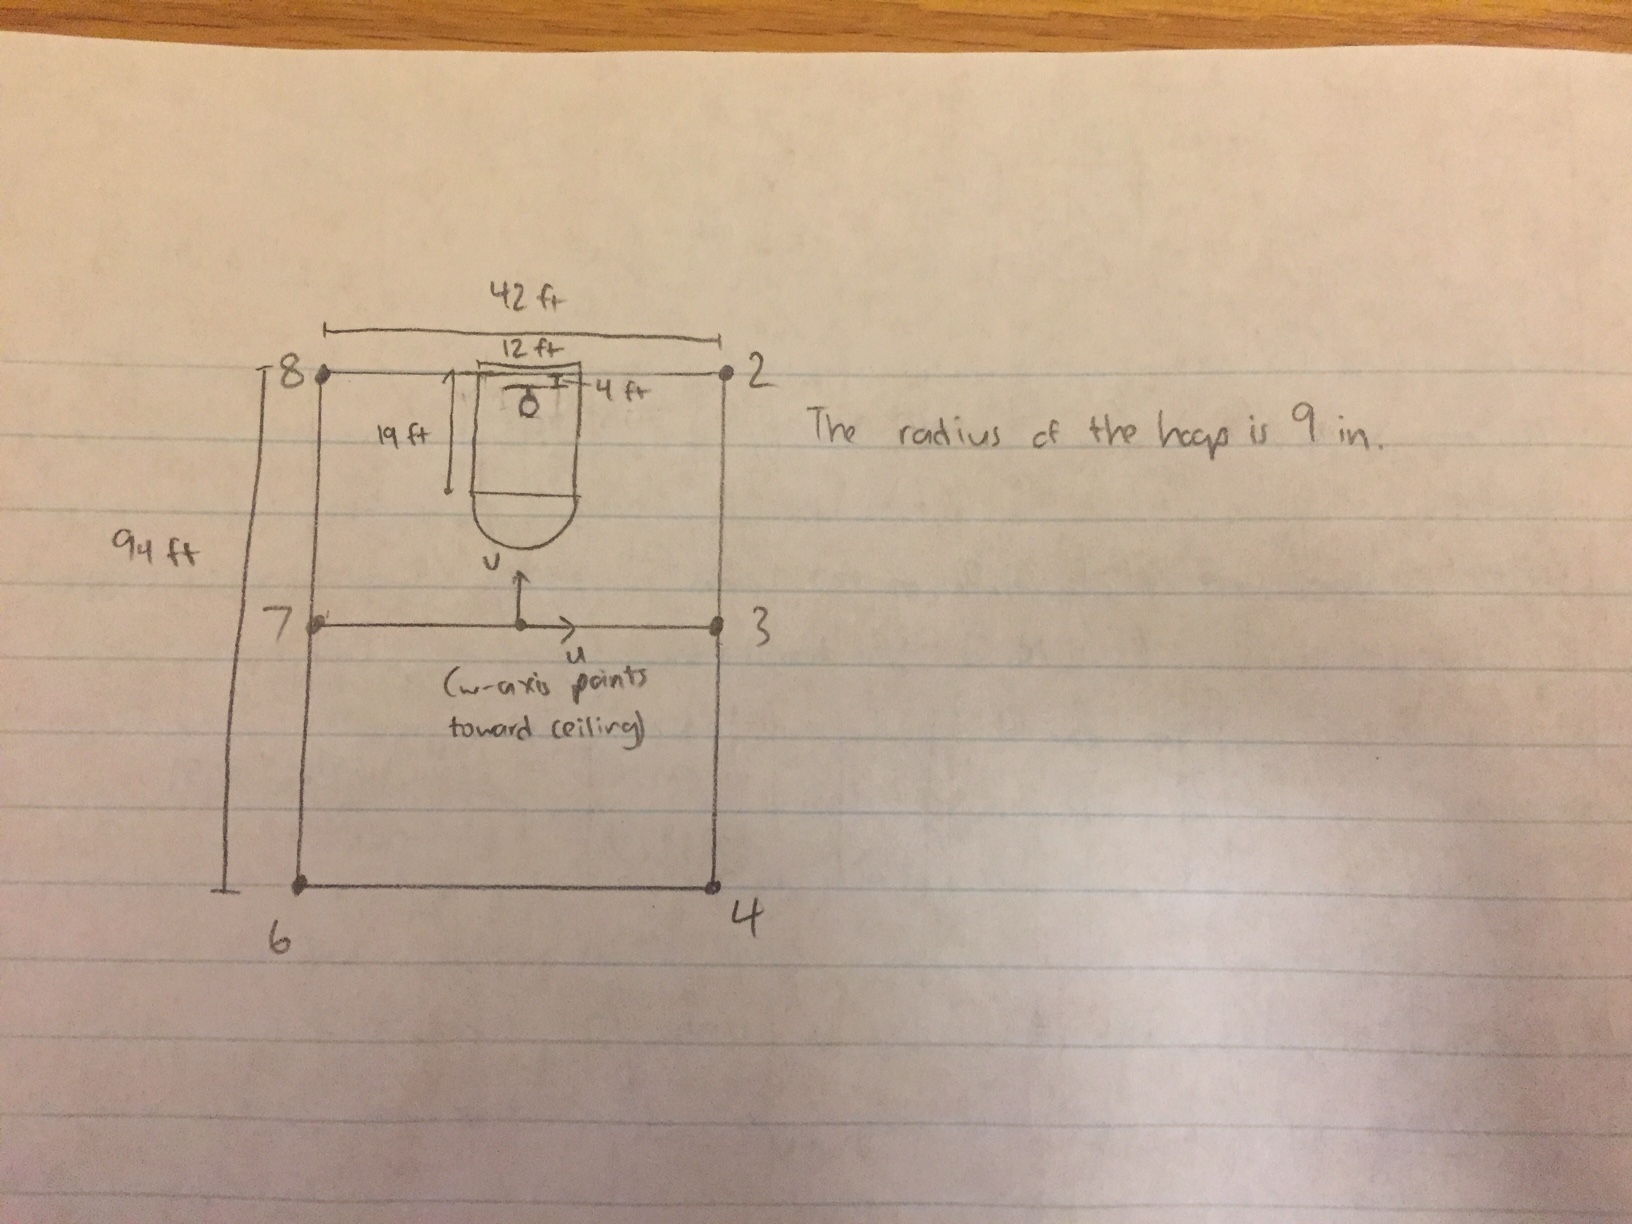
\includegraphics[scale=0.25]{Court_Diagram}
\centering
\caption{A diagram of the MAC basketball court with dimensions}
\end{figure}

For the camera frame, we will adopt the convention that the $Z$ axis points in the direction that the camera is pointing. See the following diagram, where the rectangular prism represents the camera:

\begin{figure}[H]
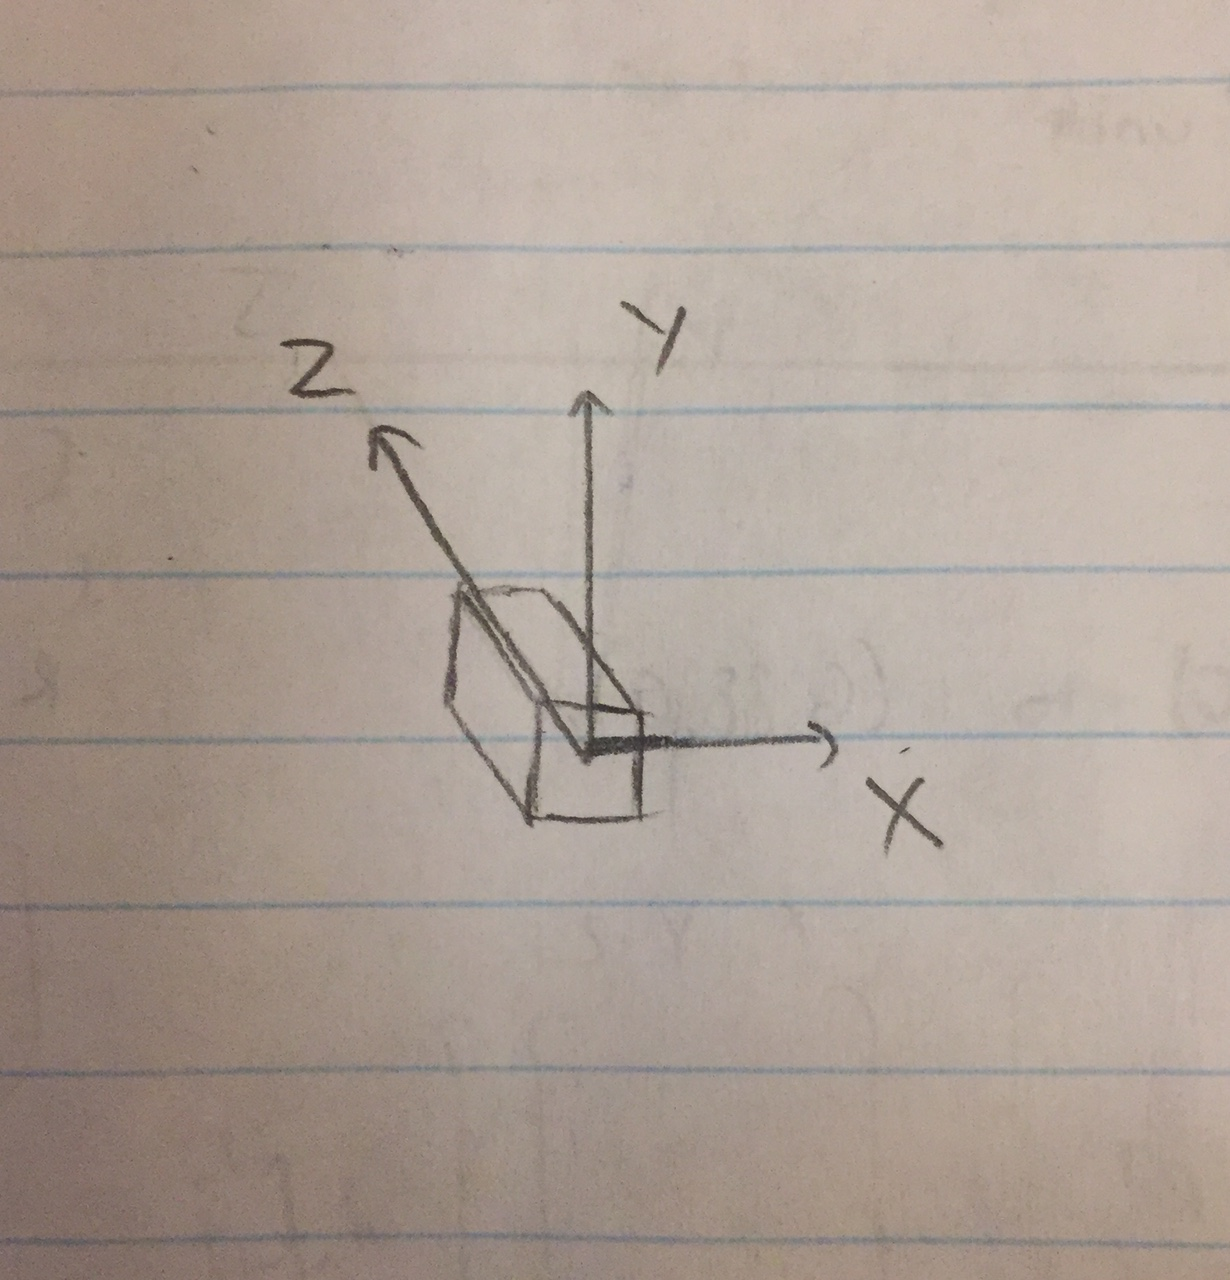
\includegraphics[scale=0.1]{Camera_Coordinates}
\centering
\caption{A poorly drawn representation of the camera coordinate system}
\end{figure}

The image coordinate system has the origin at the center of the image, with the $x$-axis pointing to the right and the $y$-axis pointing up (i.e. standard conventions). The pixel coordinate system has $(0, 0)$ representing the pixel in the top left corner. Also note that it is represented as an array in Python with the first coordinate representing the row of the pixel (so the $u$ axis points down and corresponds to the image $-y$ axis) and the second coordinate representing the column (so the $v$ axis points to the right and corresponds to the image $x$ axis).

\section{World to Camera}
To get from world coordinates to camera coordinates, we must perform a translation and then a rotation. Let the camera be placed at location $\bm{C}$ (denoting a vector) in the world frame, and let the rotation matrix be $R$. Since the rotation matrix $R$ is designed to go from the world to the camera coordinate system, $R^{T}$ is designed to go from the camera to the world. Thus, the first column of $R^{T}$ should represent the camera $X$-axis in world coordinates, the second column should represent the $Y$-axis, and the third column should represent the $Z$-axis. In terms of $R$, we see that the first \textit{row} of $R$ must be equivalent to the camera $X$-axis in world coordinates, etc. \\

In practical terms, it is relatively easy to estimate what the camera $Z$-axis is in world coordinates. By looking at one frame and identifying the center pixel (I used MS Paint for this), we can identify where in the world coordinate system the camera is pointing. The easiest way to do this is to consider where the ray pointing down the camera $Z$-axis hits a solid object. For example, if the center pixel is on the rim or the backboard, we can write a vector representing where that point is in relation to the camera position. We then normalize the vector to get the third row of $R$. \\

To get the $X$-axis, we rely on the assumption that the camera $X$-axis has a $W$-coordinate of 0 in the world frame (i.e. that it is parallel to the ground). This is a reasonable assumption because we start with the camera pointed parallel to the ground. When we tilt the camera slightly upwards, we don't rotate it in any other way, so the $X$-axis stays stationary while the $Z$ and $Y$ axes rotate (see Figure below). Thus, we look at the first two world coordinates of the camera $Z$-axis, flip the order of the coordinates, and change one sign (we flip the sign of the $U$-coordinate so that the $X$ axis points to the right). This ensures that the $X$ and $Z$ axes are orthogonal (have a dot product of 0). \\

\begin{figure}[H]
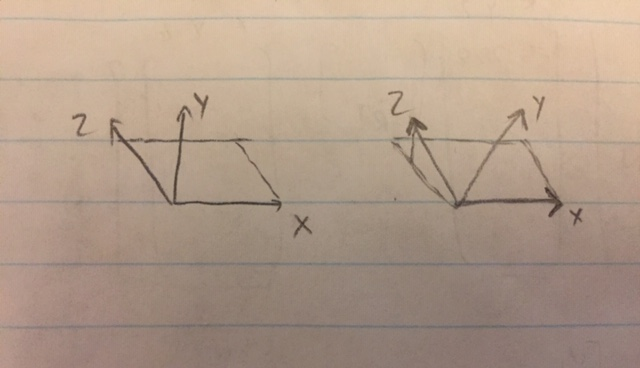
\includegraphics[scale=0.6]{Rotation_Diagram}
\centering
\caption{Why the camera $X$ axis is parallel to the ground}
\end{figure}

Finally, to get the $Y$-axis, we first normalize the $X$ and $Z$ axes, and then take the cross product of $X$ and $Z$. We make sure $X$ comes first so that the $Y$-axis points in the right direction by the right hand rule. We put our three unit vectors together and we have a rotation matrix $R$! We can now relate camera coordinates to world coordinates:

\[ \bm{P}_{C}=R(\bm{P}_{W}-\bm{C}) \]

\section{Camera to Image}
The key idea is that the ``image plane'' is an imaginary plane $f$ units down the $Z$-axis of the camera, where $f$ is the focal length. To get the image plane coordinates, we use similar triangles and scale down a point that is $Z$ units away to a plane that is $f$ units away. We get:
\begin{align*}
x&=\frac{f}{Z}X \\
y&=\frac{f}{Z}Y \\
\end{align*}

Note: Some sources like to use ``homogeneous coordinates'' so that we can write a matrix equation $\begin{bmatrix} x' \\ y' \\ z' \end{bmatrix}=\begin{bmatrix} f & 0 & 0 & 0 \\ 0 & f & 0 & 0 \\ 0 & 0 & 1 & 0 \end{bmatrix}\begin{bmatrix} X \\ Y \\ Z \\ 1 \end{bmatrix}$. Then $(x', y', z')=(Xf, Yf, Z)$ and $(x, y)=(\frac{x'}{z'}, \frac{y'}{z'})$. I don't really understand the need for this but if one of you guys wants to look into it more, please go ahead. \\

\begin{figure}[H]
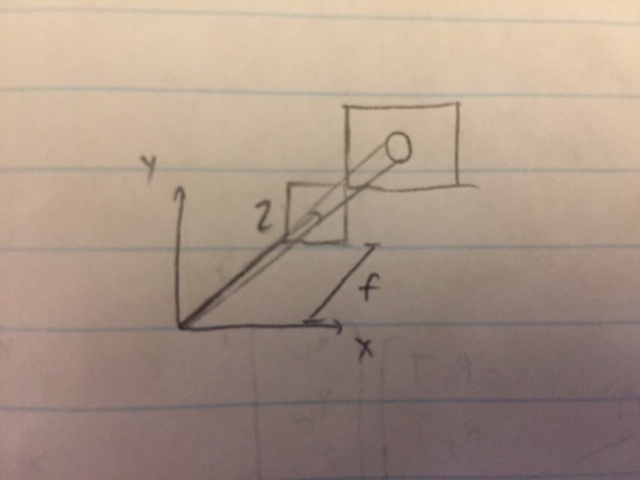
\includegraphics[scale=0.6]{Image_Plane}
\centering
\caption{Projection onto image plane}
\end{figure}

\section{Image to Pixel}
To transform from image to pixel, we have to divide the image $x$ coordinate by the width of a pixel and the image $y$ coordinate by the height of a pixel. This will tell us how many pixels away a point in the image is from the center of the image. Let the width of a pixel by $s_{x}$ and the height of a pixel by $s_{y}$. Also, note that we must negate the image $y$ coordinate because the pixel $u$ axis points down instead of up. Right now we have $u=-\frac{y}{s_y}, v=\frac{x}{s_x}$. However, we have to add $\frac{1080}{2}=540$ to $u$ and $\frac{1920}{2}=960$ to $v$ so that the pixel $(0,0)$ is in the top left corner. The exact numbers come from the fact that each frame is 1080 by 1920 pixels.

\begin{align*}
u&=-\frac{y}{s_{y}}+540 \\
v&=\frac{x}{s_{x}}+960
\end{align*}

\begin{figure}[H]
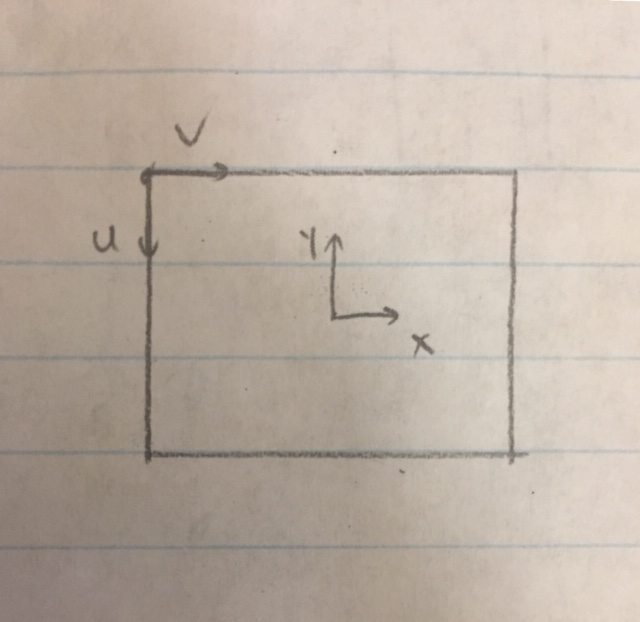
\includegraphics[scale=0.3]{Pixel_Coordinates}
\centering
\caption{Pixel coordinates vs. image coordinates}
\end{figure}

\section{Extrinsic vs. Intrinsic Parameters}
The rotation matrix $R$ and the position of the camera $\bm{C}$ are considered \textbf{extrinsic parameters} in the sense that we set them. We can also obtain good estimates of what they are without doing any algebra or optimization. On the other hand, the focal length $f$ and the pixel size $s_{x}$ by $s_{y}$ are \textbf{intrinsic parameters}, which means that they are properties of the camera. While the focal length is easily obtainable from the SOSUN website (7.36 mm unzoomed), the pixel size is unknown. However, we can estimate it using least squares! \\

We know the world coordinates of several points on the court, such as the free-throw rectangle and the white square on the backboard. Given our estimates for all of the other parameters, we can solve for the image coordinates $(x, y)$ of these points relatively easily. We can also identify the pixel coordinates $(u, v)$ of these points relatively accurately by examining a given frame (the camera is stationary). We have the equations:

\begin{align*}
v&=\frac{x}{s_{x}}+960 \\
u&=-\frac{y}{s_{y}}+540
\end{align*}

And we can write this as a matrix equation $\begin{pmatrix} v-960 \\ u-540 \end{pmatrix}=\begin{pmatrix} x & 0 \\ 0 & -y \end{pmatrix}\begin{pmatrix} \frac{1}{s_x} \\ \frac{1}{s_y} \end{pmatrix}$. We have many points where we know $(x, y)$ and $(v, u)$, so we can make this a least-squares problem where we solve for $\frac{1}{s_x}, \frac{1}{s_y}$!

\[\begin{pmatrix} v_1-960 \\ u_1-540 \\ v_2-960 \\ u_2-540 \\ \hdots \end{pmatrix}=\begin{pmatrix} x_1 & 0 \\ 0 & -y_1 \\ x_2 & 0 \\ 0 & -y_2 \\ \hdots & \hdots \end{pmatrix}\begin{pmatrix} \frac{1}{s_x} \\ \frac{1}{s_y} \end{pmatrix}\]

Assuming we have estimated all of the other parameters correctly, we should be able to get accurate numbers for $s_x, s_y$, allowing us to transform any point on the court into pixels.

\section{Alternative approaches}
We might consider solving for \textit{other} parameters using the least-squares method. However, I see two problems with this (feel free to let me know if these are valid concerns):
\begin{enumerate}
  \item Since we have $x=\frac{f}{Z}X$, etc. it is not possible to solve for our extrinsic parameters using least-squares. Our pixel coordinates are \textit{non-linear} functions of the elements in the rotation matrix $R$ and translation vector $\bm{C}$.
  \item Solving for these extrinsic parameters using least-squares might result in results that don't make physical sense. We might find that the residual is smallest with some rotation matrix that might be numerically valid but represents a physical situation in which the camera is not pointed anywhere near the hoop.
\end{enumerate}

\section{An example, using Camera 3}
Using Camera 1, we can see that Camera 3 is outside of the court, slightly behind and to the right of where it is supposed to be on the diagram. We also know that it is on a 5-foot high tripod. Using the diagram of the court, we estimate that its position relative to the world-frame origin is $\bm{C}=(22, -1.5, 5.2)$. \\

Next, we compute the rotation matrix. The center pixel of frame 20 (we could choose any frame) lies directly below the front of the rim. If we draw a line from the rim to the ground (using MS Paint), we estimate that the camera is pointed about 2 feet below the front of the rim. The point 2 feet below the front of the rim has world coordinates $(0, 41, 8)$, so the camera $z$-axis points in the direction $(-22, 42.5, 2.8)$. Our assumption is that the $x$-axis has a 3rd coordinate of 0 and points towards the northeast, so it must be of the form $(42.5, 22, 0)$ in order to be orthogonal to $z$ (of course, it could be any scalar multiple of this). In Python, we normalize our two vectors and then take $x\times z$ to get the $y$-axis. Our rotation matrix is $R=\begin{pmatrix} \vec{x}_n \\ \vec{y}_n \\ \vec{z}_n \end{pmatrix}$ where the $n$ subscript indicates that our vectors are normalized to have norm 1. \\

Note that our choice to look at the point 2 feet below the front of the rim was arbitrary, as the camera $z$-axis represents a ray. However, it was the easiest choice because it was a point on the ray with coordinates that were relatively easy to estimate. \\

From here, all we need to do is solve the least-squares point for the pixel size $(s_x, s_y)$. For our ``known'' points, we take the free throw rectangle and the white box on the backboard. The four corners of the free throw rectangle are $(-6, 28, 0), (-6, 47, 0), (6, 47, 0), (6, 28, 0)$ in world coordinates, and the four corners of the box on the backboard are $(-1, 43, 10), (-1, 43, 11.5), (1, 43, 11.5), (1, 43, 10)$. We also consider some intermediate points on the free throw rectangle (I used all of the points with integer coordinates). Using Python, we can create a $N$ by 3 matrix with the world coordinates of these points. With the parameters we already know, we can construct the 2D image plane coordinates of these points. \\

We can also get the pixel coordinates of all of our points with reasonable accuracy by looking at the photo in MS Paint or similar software. I did this by getting the pixel coordinates of the corners and using linspace. Now that we have our pixel coordinates and our 2D image plane coordinates for all of our points, we solve the least squares problem for $s_x$ and $s_y$. Our final step in Python is to use our estimated values of $s_x$ and $s_y$ to complete the transformation and color the pixels corresponding to our real-world points (in this case, the free throw rectangle and the white box).

\section{Software package}
There is a package called OpenCV that also exists in Python. It seems to have something to do with tracking objects using a camera. However, it might be do all of the underlying math for us and defeat the purpose of our project.

\bigskip
\section{Resources}
\url{http://www.cse.psu.edu/~rtc12/CSE486/lecture12.pdf} \\
\url{http://www.cse.psu.edu/~rtc12/CSE486/lecture13.pdf} \\
\url{https://courses.cs.washington.edu/courses/cse455/09wi/Lects/lect5.pdf} \\
\url{https://www.cs.utah.edu/~srikumar/cv_spring2017_files/Lecture2.pdf} \\
\url{http://www.cs.toronto.edu/~jepson/csc420/notes/imageProjection.pdf} \\
\url{http://people.scs.carleton.ca/~c_shu/Courses/comp4900d/notes/camera_calibration.pdf} \\
\url{http://www.cs.ucf.edu/~mtappen/cap5415/lecs/lec19.pdf} \\
\url{https://www.cse.unr.edu/~bebis/CS791E/Notes/CameraParameters.pdf} \\














\end{document}